\subsubsection{Introduction to Induction}

\begin{frame}<beamer>{Structure}
  \tableofcontents[currentsection,currentsubsection]
\end{frame}

\begin{frame}{Induction}
  \textbf{Basics:}
  \begin{itemize}
    \item
      You want to show assumption $A(n)$ is valid $\forall n \in \mathbb{N}$
    \item
      We show induction in two steps:
      \begin{enumerate}
        \item
          \textbf{Induction basis:} we show that our assumption is valid 
          at one point (for example: $n = 1$).
        \item
          \textbf{Induction step:} we show that the assumption is valid for 
          all $n$ (normally one step forward: $n = n + 1$).
      \end{enumerate}
    \item
      If both has been proven, then {\color{MainA}$A(n)$} holds for all natural
      numbers {\color{MainA}$n$} by \textbf{induction}
  \end{itemize}
\end{frame}

%-------------------------------------------------------------------------------

\begin{frame}{Induction - Example 1}
  \begin{block}{Claim:}
    A \textbf{complete} binary tree of depth $d$ has $n(d) = 2^d - 1$ nodes
  \end{block}
  \begin{itemize}
    \item
      \textbf{Induction basis:} Formular holds for {\color{MainA}$d = 1$}
      \begin{columns}
        \begin{column}{0.5\linewidth}
          \begin{figure}[!h]
            \begin{adjustbox}{width=4em}
              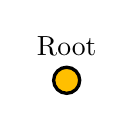
\begin{tikzpicture}[
  level/.style={
    sibling distance = 10.0em/#1,
    level distance = 3.5em
  },
  node/.style={
    draw,
    circle,
    very thick,
    color=black,
    fill=white
  },
  node_filled/.style={
    node,
    color=black,
    fill=orange!50!yellow
  }
]%
\node [node_filled, label={[anchor=south]above:Root}] (root) {};
\end{tikzpicture}
            \end{adjustbox}
            \caption{Tree of depth {\color{MainA}$1$} has
              {\color{MainA}$1$} node}
          \end{figure}
        \end{column}
        \begin{column}{0.5\linewidth}
          {\color{MainA}$n(1) = 2^1 - 1 = 1$}\\
          $\Rightarrow$ correct $\checkmark$
        \end{column}
      \end{columns}
  \end{itemize}
\end{frame}

%-------------------------------------------------------------------------------

\begin{frame}{Induction - Example 1}
  Number of nodes $n(d)$ in a binary tree with depth $d$:
  \begin{itemize}
    \item
      \textbf{Induction assumption:}
      {\color{MainA}$n(d) = 2^d-1$}
    \item<2- |handout:1>
      \textbf{Induction basis:}
      $n(1) = 2^d - 1 = 2^1 - 1 = 1 ~{\color{Mittel-Blau}\checkmark}$
    \item<3- |handout:1>
      \textbf{Induction step:}
      to show for $d = d + 1$
      \begin{columns}
        \begin{column}<3- |handout:1>{0.6\textwidth}
          \begin{figure}%
            \begin{adjustbox}{height=7.0em}
              \tikzstyle{node}=[
  draw,
  circle,
  very thick,
  color=black,
  fill=white
]%
%
\tikzstyle{node_tree}=[
  draw,
  circle,
  very thick,
  color=black,
  fill=white
]%
%
\tikzstyle{tree}=[
  draw,
  very thick,
  shape border uses incircle,
  isosceles triangle,
  shape border rotate=90,
  yshift=-4em,
  color=black,
  fill=green!50!white,
  minimum height=8.0em
]%
%
\tikzstyle{path}=[
  draw,
  very thick,
  color=black
]%
%
\tikzstyle{brace}=[
  very thick,
  color=black,
  decoration={
    brace,
    raise=0.75em,
    amplitude=15pt
  },
  decorate
]%
%
\tikzstyle{line}=[
draw,
loosely dotted,
very thick,
color=black
]%
\begin{adjustbox}{height=7.0em}
\begin{tikzpicture}[
  level/.style={
    sibling distance = 8.0em,
    level distance = 1.5em
  }
]
\node [node, label={[anchor=south]above:Root}] (root) {}
child [path] {
  child {
    node[tree] {{\protect\onslide<4->{\Large $n(d)$}}}
  }
  node [node_tree] {}
}
child [path] {
  child {
    node[tree] {{\protect\onslide<4->{\Large $n(d)$}}}
  }
  node [node_tree] {}
};
% --------------------------------- left brace ---------------------------------
\draw (-2.75, -3.5) [brace] -- node [
  color=black,
  pos=0.5,
  xshift=-3.5em,
  rotate=90,
  font=\huge
] {$d+1$} (-2.75, 0.0);
\draw (-2.75, 0.0) [line] -- (-0.5, 0.0);
% --------------------------------- right brace --------------------------------
\draw (2.75, -3.5) [brace,decoration={mirror}] -- node [
  color=black,
  pos=0.5,
  xshift=3.5em,
  rotate=90,
  font=\huge
] {$d$} (2.75, -0.5);
\draw (2.75, -0.5) [line] -- (2.0, -0.5);
\end{tikzpicture}
\end{adjustbox}%
            \end{adjustbox}%
            \vspace{-0.5em}
            \caption{Binary tree with subtrees}%
            \label{fig:binary_tree_subtrees}%
          \end{figure}
        \end{column}
        \begin{column}{0.4\linewidth}
          \vspace{1.5em}
          \begin{align*}
            \onslide<4- |handout:1>{
              n(d + 1) = &~ 2 \cdot n(d) + 1
            }\\
            \onslide<5- |handout:1>{
              {} = &~ 2 \cdot \textcolor{MainA}{\left(2^d - 1\right)} + 1
            }\\
            \onslide<6- |handout:1>{
              {} = &~ 2^{d + 1} - 2 + 1
            }\\
            \onslide<7- |handout:1>{
              {} = &~ 2^{d + 1} - 1 ~{\color{MainA}\checkmark}
            }
          \end{align*}
          \onslide<8- |handout:1>{
            \llap{$\Rightarrow$ \textbf{By induction:}}
            $n(d) = 2^d - 1 ~\forall n \in \mathbb{N} ~\Square$
          }
        \end{column}
      \end{columns}
  \end{itemize}
\end{frame}

%-------------------------------------------------------------------------------

\begin{frame}{Induction - Example 2}
  \begin{itemize}
    \item
      \textbf{Induction assumption:}
      \begin{align*}
        {\color{Hell-Gruen}A}(n) \leq &~ {\color{Hell-Gruen}B}(n)\\
        \sum \limits^n_{i=1} \left(i \cdot 2^{n-i} \right) \leq &~ 2^{n+1}
      \end{align*}
    \item
      \textbf{Induction basis:}
      $n = 1$:
      \begin{align*}
        \sum \limits^n_{i=1} \left(i \cdot 2^{n-i} \right) \leq &~ 2^{n+1}\\
        \sum \limits^1_{i=1} \left(i \cdot 2^{1-i} \right) \leq &~ 2^{1+1}\\
        2^0 \leq &~ 2^2 ~{\color{Mittel-Blau}\checked}
      \end{align*}
  \end{itemize}
\end{frame}

%-------------------------------------------------------------------------------

\begin{frame}{Induction - Example 2}
  \textbf{Induction step:}
  $(n = n +1)$:
  \begin{align*}
    {\color{Hell-Gruen}A}(n+1) \leq &~ {\color{Hell-Gruen}B}(n+1)\\
    %----------------------------------------------------------------------
    \sum\limits^{n+1}_{i=1} \left(i \cdot 2^{n+1-i} \right)
    \leq &~ 2^{n+1+1}\\
    %----------------------------------------------------------------------
    2 \cdot \sum\limits^{n+1}_{i=1} \left(i \cdot 2^{n-i} \right)
    \leq &~ 2 \cdot 2^{n+1} & \hspace*{1.5em} \bigg\vert :2\\
    %----------------------------------------------------------------------
    \sum\limits^{n+1}_{i=1} \left(i \cdot 2^{n-i} \right)
    \leq &~ 2^{n+1}\\
  \end{align*}
\end{frame}

%-------------------------------------------------------------------------------

\begin{frame}{Induction - Example 2}
  \textbf{Induction step:}
  $(n = n +1)$:
  \begin{align*}
    \sum\limits^{n+1}_{i=1} \left(i \cdot 2^{n-i} \right)
    \leq &~ 2^{n+1}\\
    %----------------------------------------------------------------------
    \sum\limits^{n}_{i=1} \left(i \cdot 2^{n-i}\right)
    + \left(n + 1\right) \cdot 2^{n - \left(n + 1\right)}
    \leq &~ 2^{n+1}\\
    %----------------------------------------------------------------------
    \sum\limits^{n}_{i=1} \left(i \cdot 2^{n-i}\right)
    + 2n + 2
    \leq &~ 2^{n+1}\\
    %----------------------------------------------------------------------
   {\color{Hell-Gruen}A}(n) + 2n + 2
   \leq &~ {\color{Hell-Gruen}B}(n) ~\textbf{\color{Mittel-Blau}\lightning}
  \end{align*}
  \begin{center}
    \alert{Assumtion is still correct!}
  \end{center}
\end{frame}